\documentclass{standalone}
\usepackage{tikz}
\usepackage{ctex,siunitx,upgreek}
\setCJKmainfont{Noto Serif CJK SC}
\usepackage{tkz-euclide}
\usepackage{amsmath}
\usetikzlibrary{patterns, calc,3d}
\usetikzlibrary {decorations.pathmorphing,decorations.pathreplacing,decorations.shapes}
\begin{document}
\small
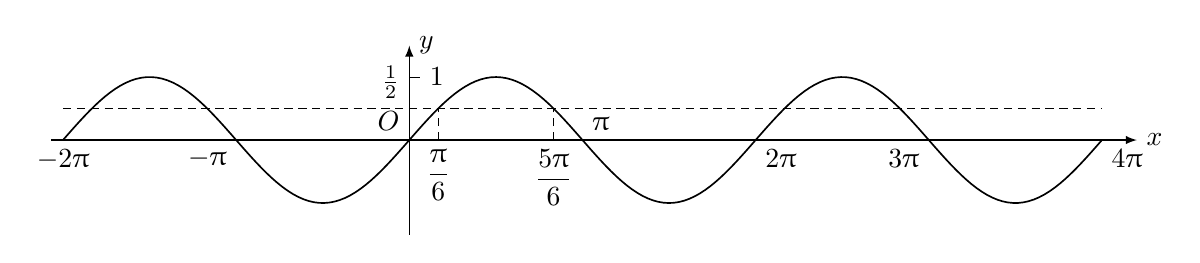
\begin{tikzpicture}[>=latex,xscale=0.7,yscale=0.8]
  \draw[->](-6.5,0)--(13.2,0)node[right]{$x$};
  \draw[->](0,-1.5)--(0,1.5)node[right]{$y$};
  \node at (0,0)[above left]{$O$};
  \draw[semithick,samples=200,domain=-2*pi:4*pi] plot (\x,{sin(\x r)});
  \draw[densely dashed](-2*pi,0.5)--(4*pi,0.5)(pi/6,0)--(pi/6,0.5)(5*pi/6,0)--(5*pi/6,0.5);
  \node at (-2*pi,0)[below ]{$-2\uppi$};
  \node at (0,0.5)[above left]{$\frac12$};
  \draw [very thin](0,1)--(0.2,1)node[right]{1};
  \node at (-pi,0)[below left]{$-\uppi$};
  \node at (2*pi,0)[below right]{$2\uppi$};
  \node at (4*pi,0)[below right]{$4\uppi$};
  \node at (3*pi,0)[below left]{$3\uppi$};
  \node at (pi,0)[above right]{$\uppi$};
  \node at (pi/6,0)[below]{$\dfrac\uppi6$};
  \node at (5*pi/6,0)[below]{$\dfrac{5\uppi}{6}$};
\end{tikzpicture}
\end{document}